\section {Lepton and B-jet Overlap Removal: Impact On Signal Efficiency}
\label{app:bjetlepOR}

The overlap removal procedure, as presented in Sec.~\ref{sec:overlapremoval} requires calorimeter-jets to 
be removed from the event if it is within. Due to the presence of $b$-jets from the $h \to b\bar{b}$ decay,
it is possible for a reconstructed muon or electron to be in close proximity of the $b$-jets, due to semi-leptonic
decays of the $b$-hadron, and the $b$-jets fail the overlap removal criteria. Figure~\ref{fig:bjetlepOR} shows
the signal efficiency to find the leading and sub-leading $b$-jet in the event. In this study, 
the $b$-jets are identified by requiring at least one $b$-hadron within the $b$-jets. 

The efficiency loss due to electrons, which pass the VHLooseElectron selection, 
to be within $\Delta R$ < 0.2 of the b-jets are negligible as can be seen in the top figures. 
For muons that pass VHLooseMuon selection, the impact is slightly more pronounced but still small ($\sim$3\%). 
Note that in the jet-muon overlap removal procedure, additional requirements are imposed on the muon and 
the overlapping jet before deciding to remove the jet and this is expected to mitigate the lost of efficiency.
The impact of the additional requirements are not studied here.

\begin{figure}[!h]
\begin{center}
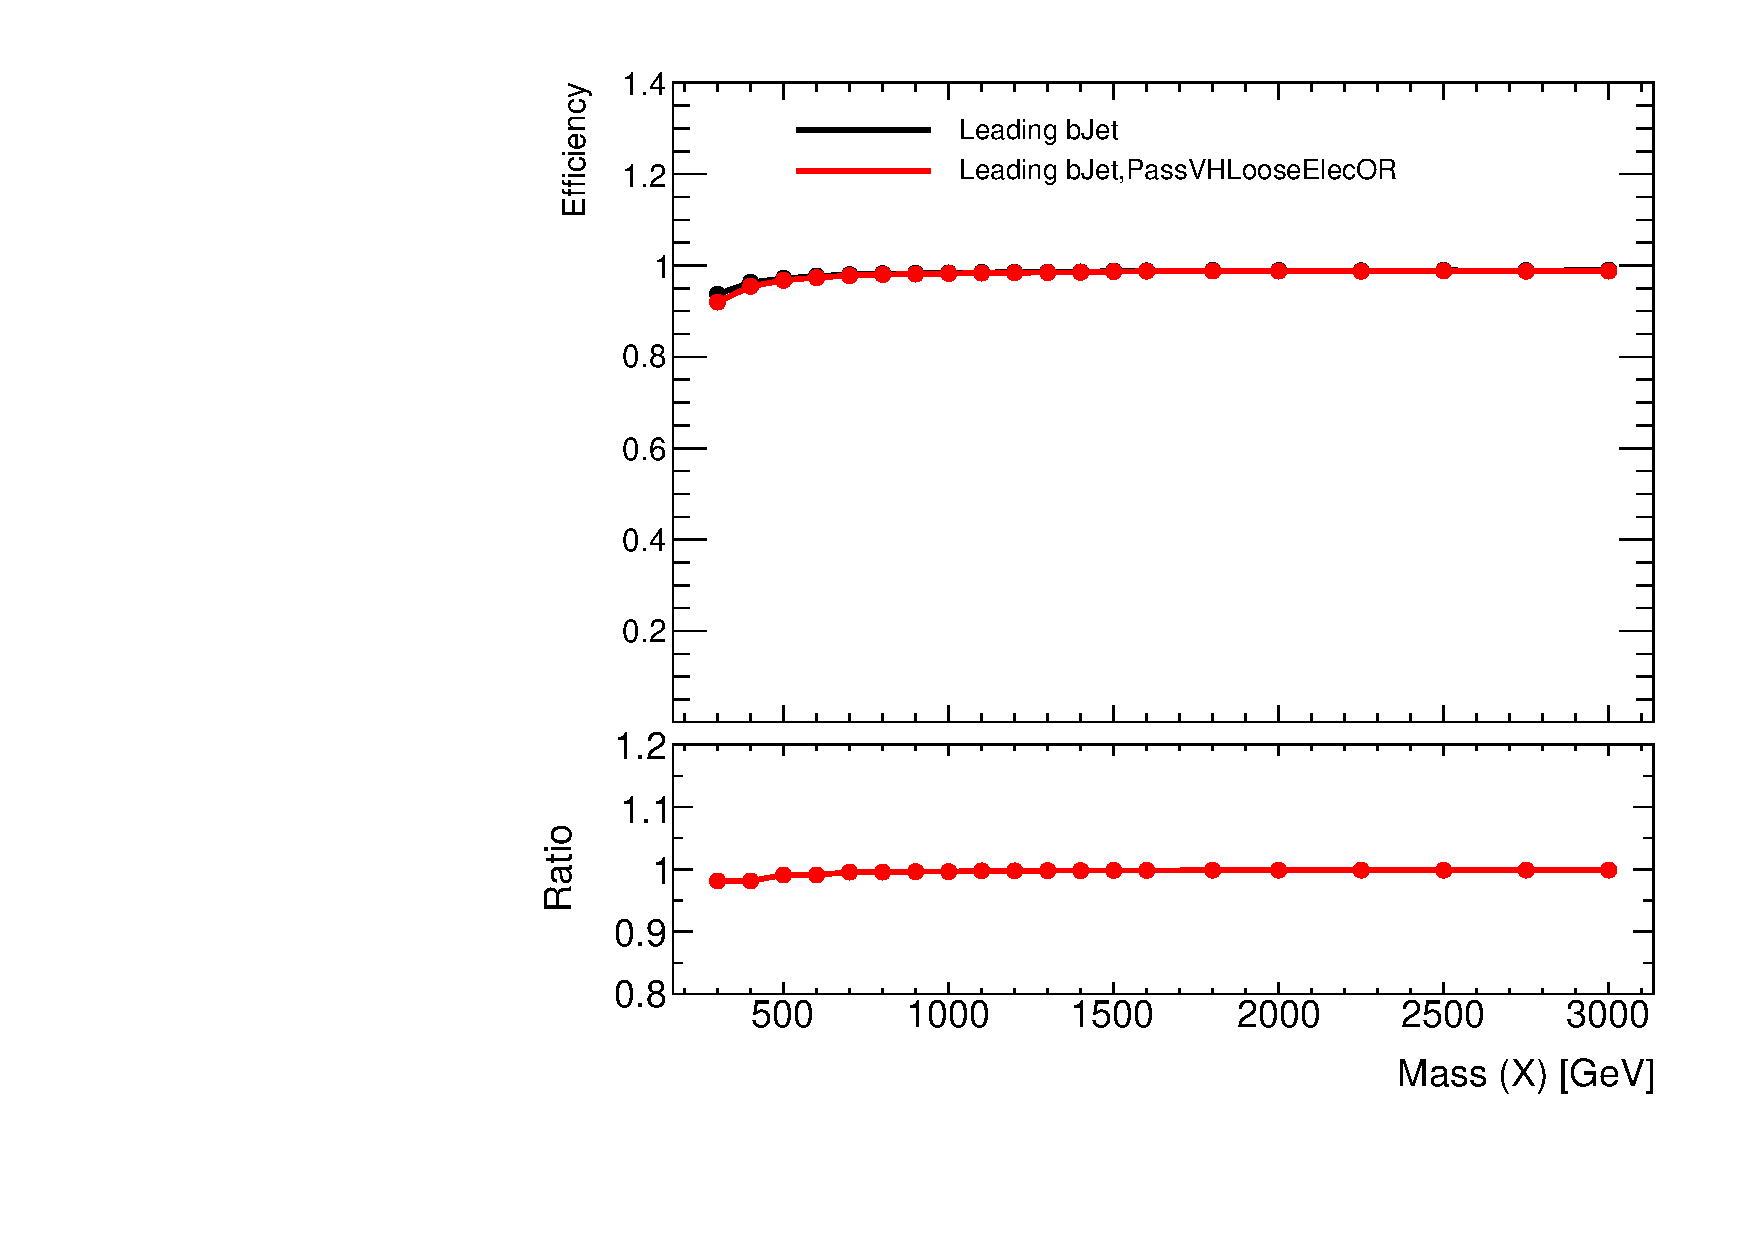
\includegraphics[width=0.49\textwidth] {figures/app-bjetleptonoverlap/looseElec_trubcentraljet0}
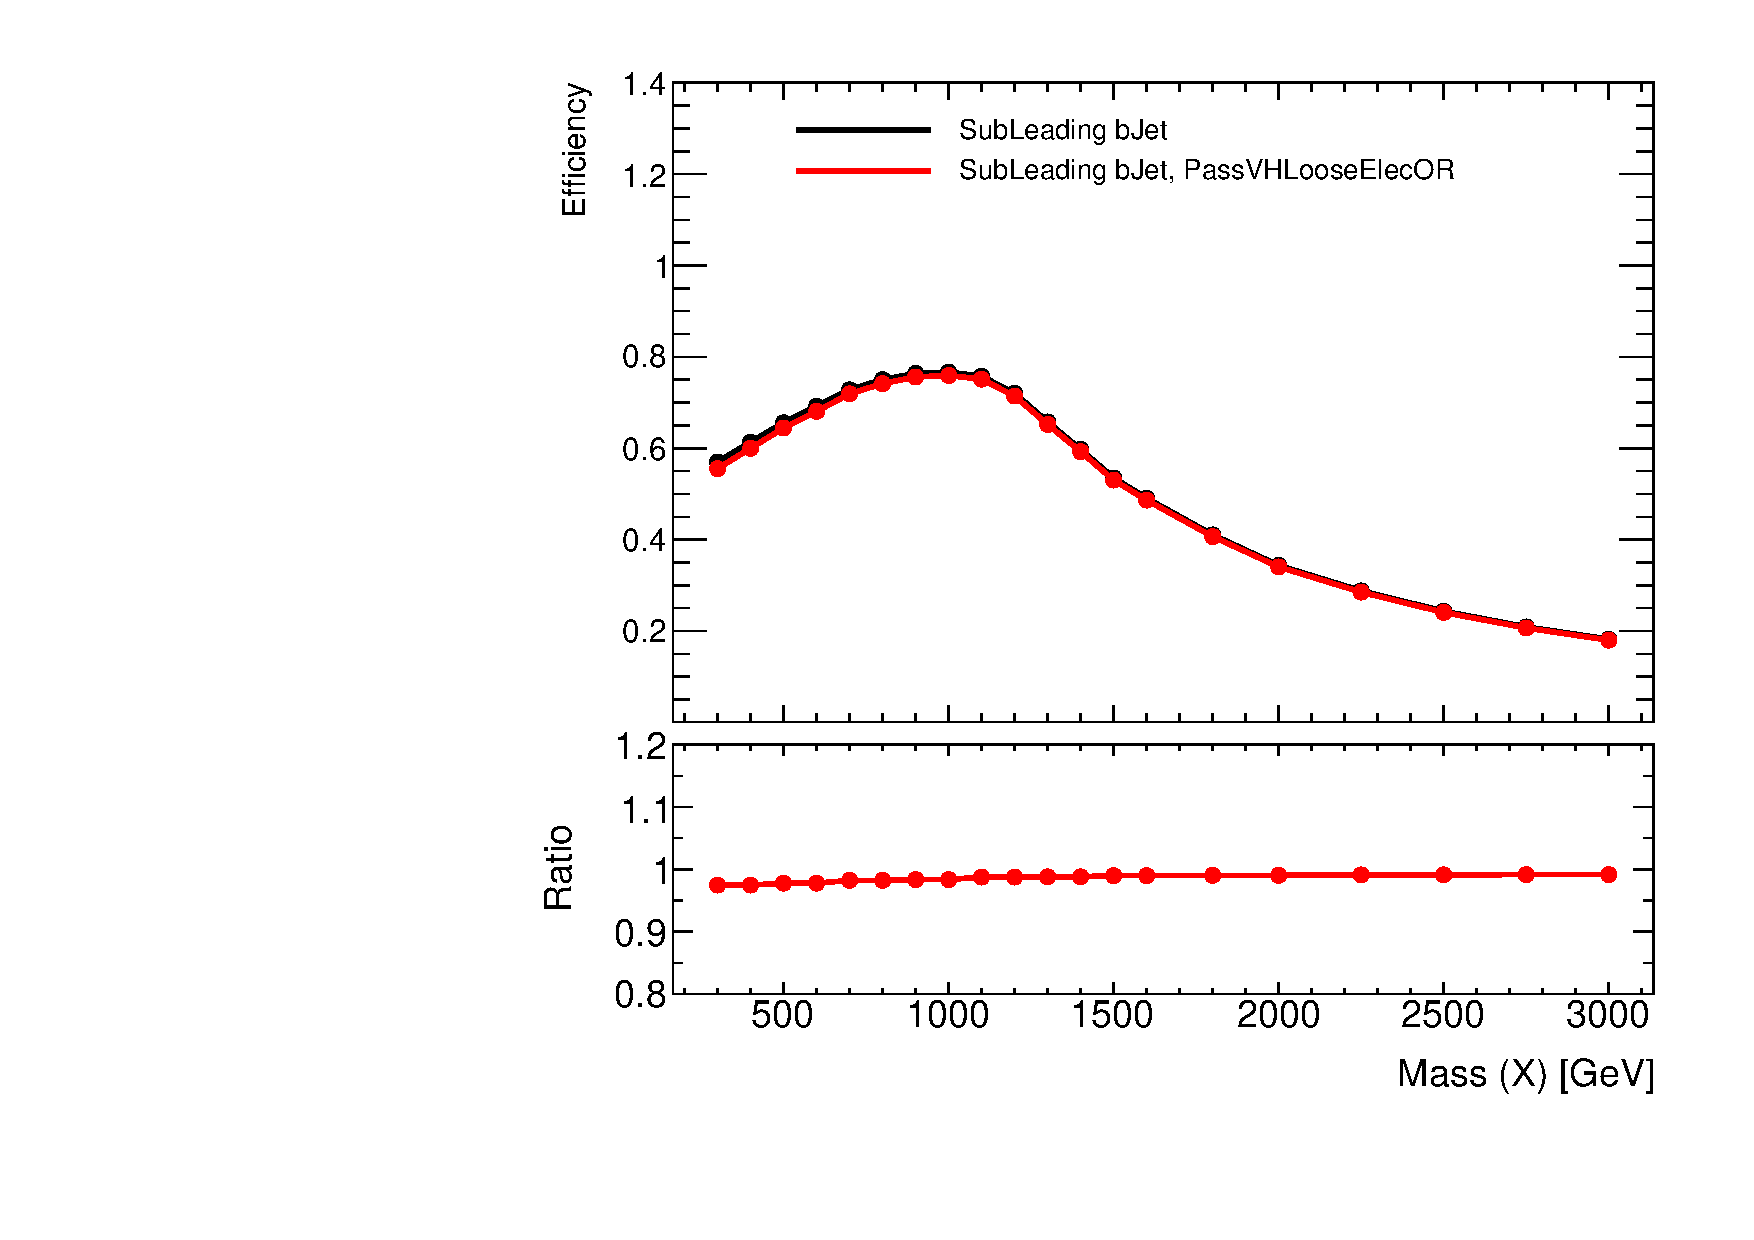
\includegraphics[width=0.49\textwidth] {figures/app-bjetleptonoverlap/looseElec_trubcentraljet1}\\
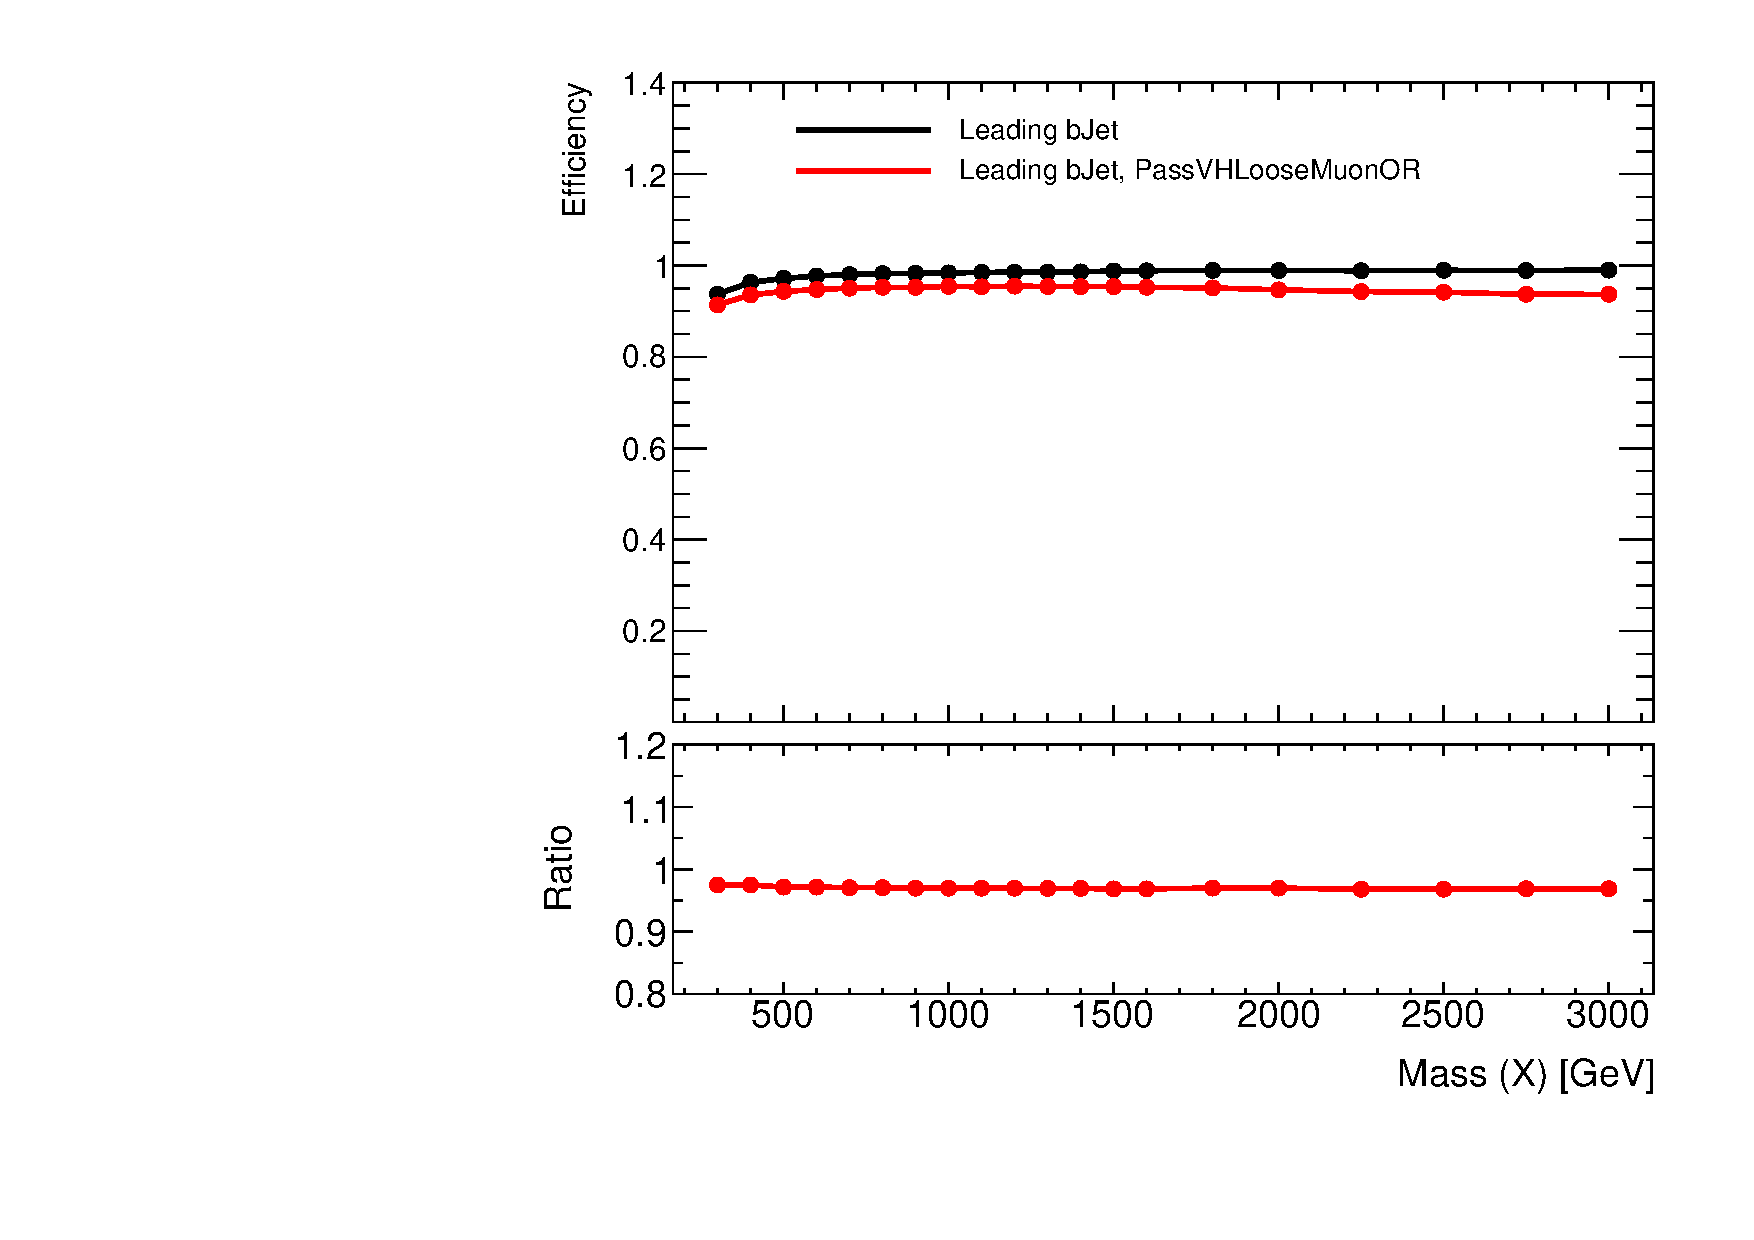
\includegraphics[width=0.49\textwidth] {figures/app-bjetleptonoverlap/looseMuon_trubcentraljet0}
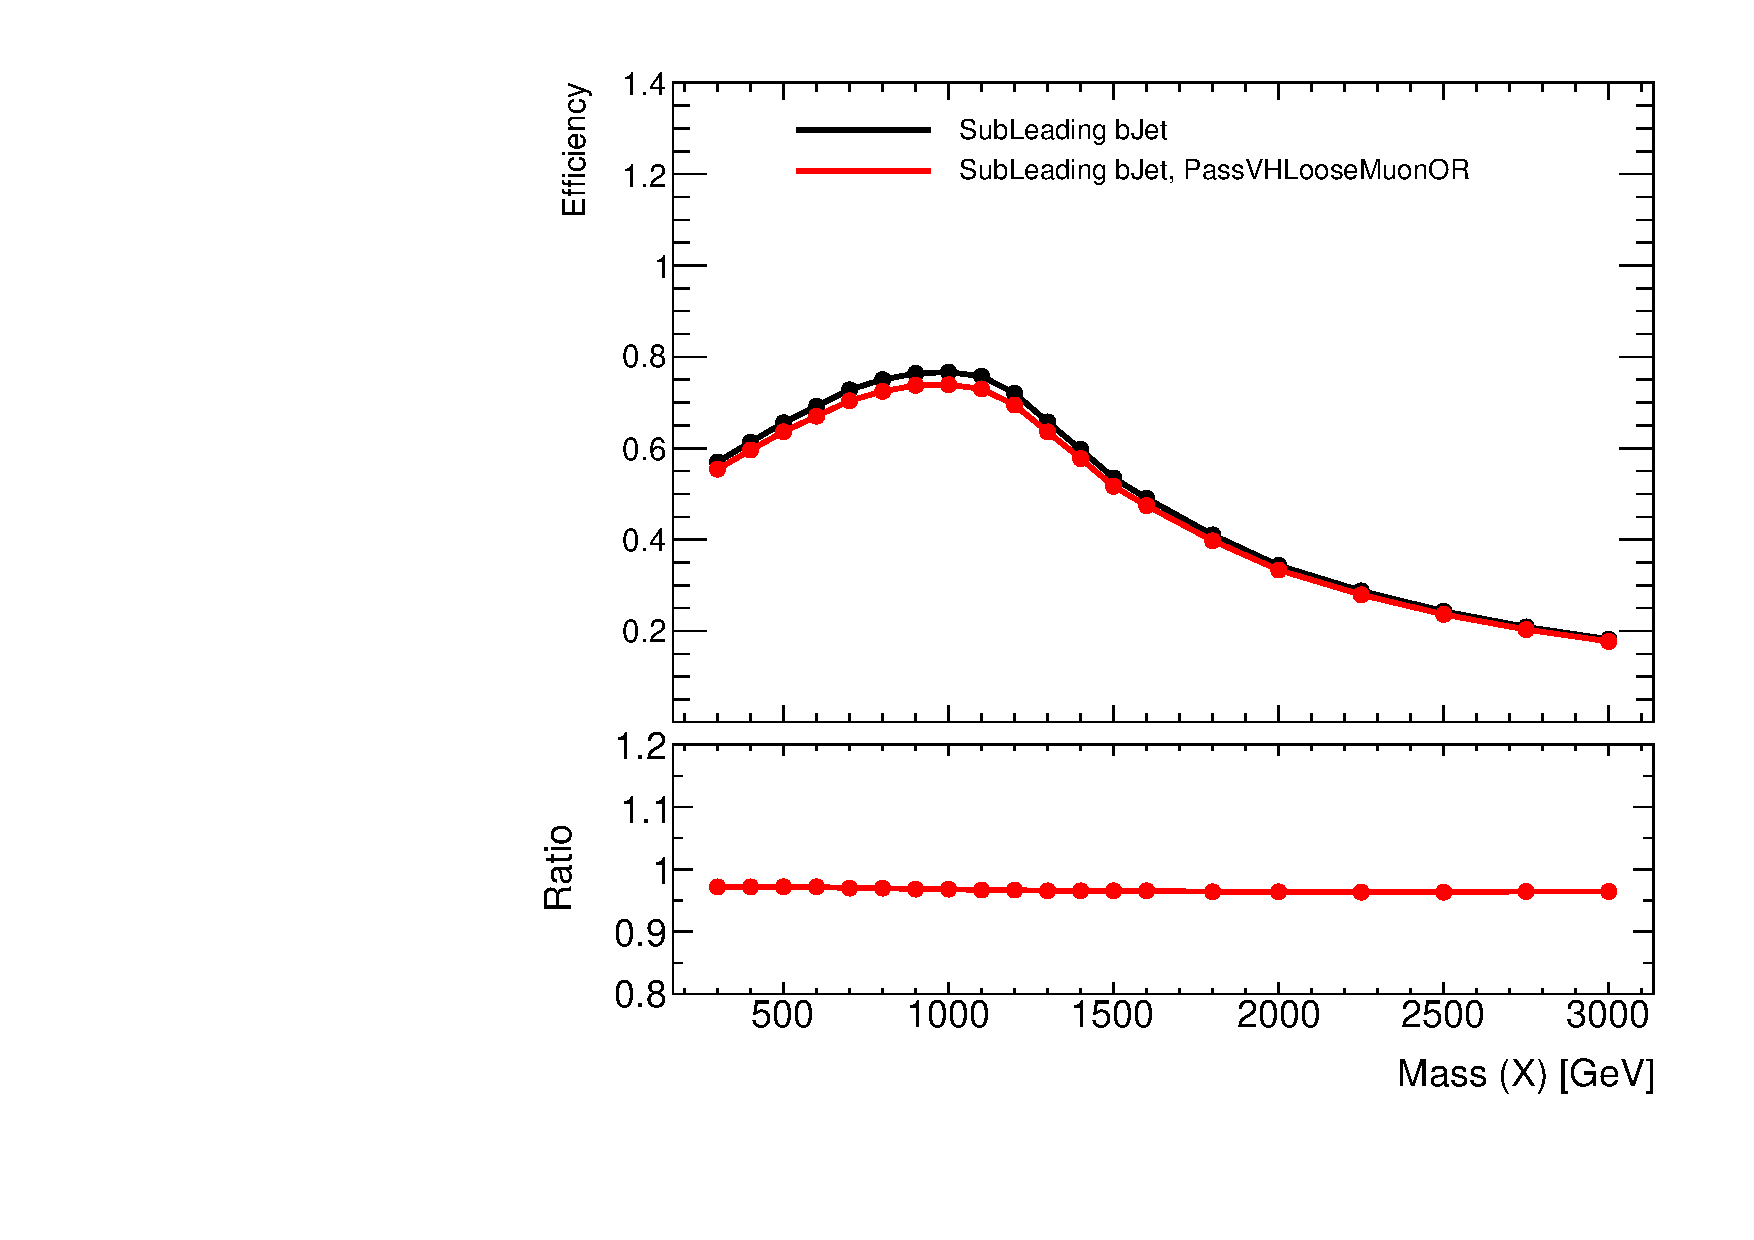
\includegraphics[width=0.49\textwidth] {figures/app-bjetleptonoverlap/looseMuon_trubcentraljet1}
\caption[]{The signal efficiencies to find the leading (left) and sub-leading (right) jets
which has at least 1 $b$-hadron within the jets. The red curves correspond to the requirement that 
the jets do not have a VHLoose electrons (top) and muons (bottom) within $\Delta R$ < 0.2 from the jet axis. 
}
\label{fig:bjetlepOR}
\end{center}
\end{figure}
